%\documentclass[fleqn, letterpaper]{amsart}
\documentclass[letterpaper]{tufte-handout}
\usepackage{times}
\usepackage{amsmath}
\usepackage{amssymb}
\usepackage{graphicx}
\usepackage{booktabs}
\usepackage{multirow}
\usepackage{listings}
\usepackage{epstopdf}
\usepackage{bm}
\usepackage{natbib}
%\usepackage[left=1in]{geometry}

\newcommand{\R}{\mathcal{R}}
\newcommand{\E}{\text{E}}
\newcommand{\p}{p_{XY}}
\newcommand{\T}{^\text{T}}
\newcommand{\y}{\mathbf{y}}
\newcommand{\z}{\mathbf{z}}
\newcommand{\I}{\mathbf{I}}
\newcommand{\HH}{\mathbf{H}}
\newcommand{\A}{\mathbf{A}}
\newcommand{\GG}{\mathbf{G}}
\newcommand{\vecv}{\mathbf{v}}
\newcommand{\uu}{\mathbf{u}}
\newcommand{\cyy}{\mathbf{C}_{yy}}
\newcommand{\cyz}{\mathbf{C}_{yz}}
\newcommand{\czz}{\mathbf{C}_{zz}}
\newcommand{\cuu}{\mathbf{C}_{uu}}
\newcommand{\cvv}{\mathbf{C}_{vv}}
\newcommand{\cpp}{\mathbf{C}_{\psi\psi}}
\renewcommand{\arraystretch}{1.5}
\newcommand{\KK}{\left(\begin{array}{c} \frac{{\sigma_{\y_1}}^2}{{\sigma_v}^2 + {\sigma_{\y_1}}^2}\\ \frac{\sigma_{\y_1\y_2}}{{\sigma_v}^2 + {\sigma_{\y_1}}^2} \end{array}\right)}
\newcommand{\cyylong}{\left(\begin{array}{cc} {\sigma_{y_1}}^2 & \sigma_{\y_1\y_2}\\ \sigma_{\y_1\y_2} & {\sigma_{y_2}}^2 \end{array}\right)}
\renewcommand{\vec}[1]{\mathrm{#1}}

\title{Problem Set 8 --- ENCE689E Spring 2014}
\author{David Prentiss}

\begin{document}
\maketitle

\section{1. Precipitation Errors}
\subsection{(a)}
\begin{figure}
  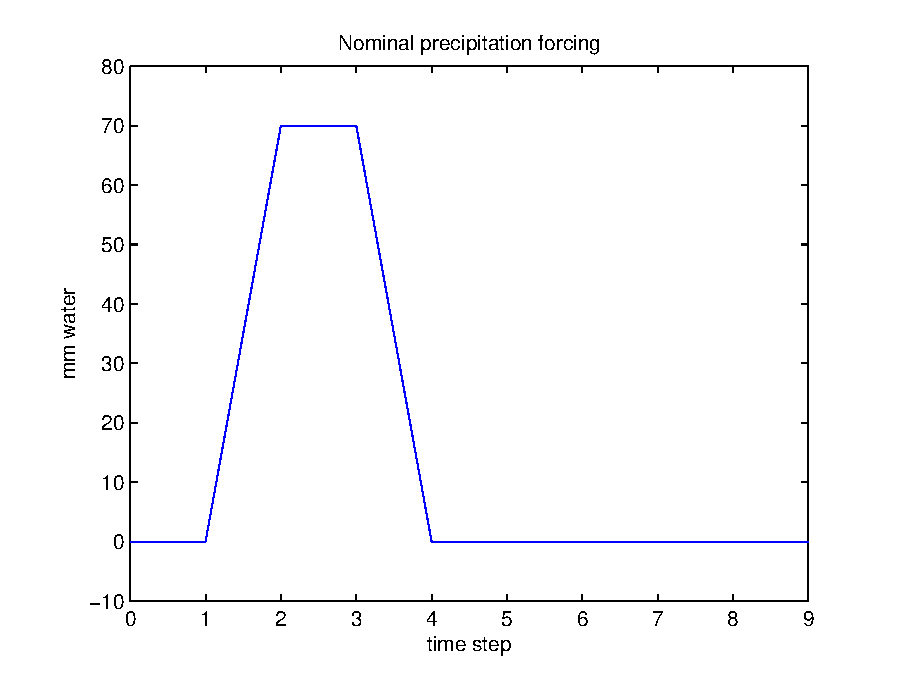
\includegraphics[width=\textwidth]{1a}
  \caption{Nominal precipitation forcing from Problem Set 5.}
  \label{1b}
\end{figure}
\subsection{(b)}
\begin{itemize}
  \item For the unbiasedness assumption, the mean of the additive error must be zero.
  \item A ten--member ensemble was generated with the code in Listing \ref{list1b} and plotted in Figure \ref{1b}.
    {\small
    \lstinputlisting[language=Matlab, caption={Ten--memeber, precipitation forcing ensemble.},
    basicstyle=\ttfamily, label=list1b]{ps8_1.m}
  }
    \begin{figure}
      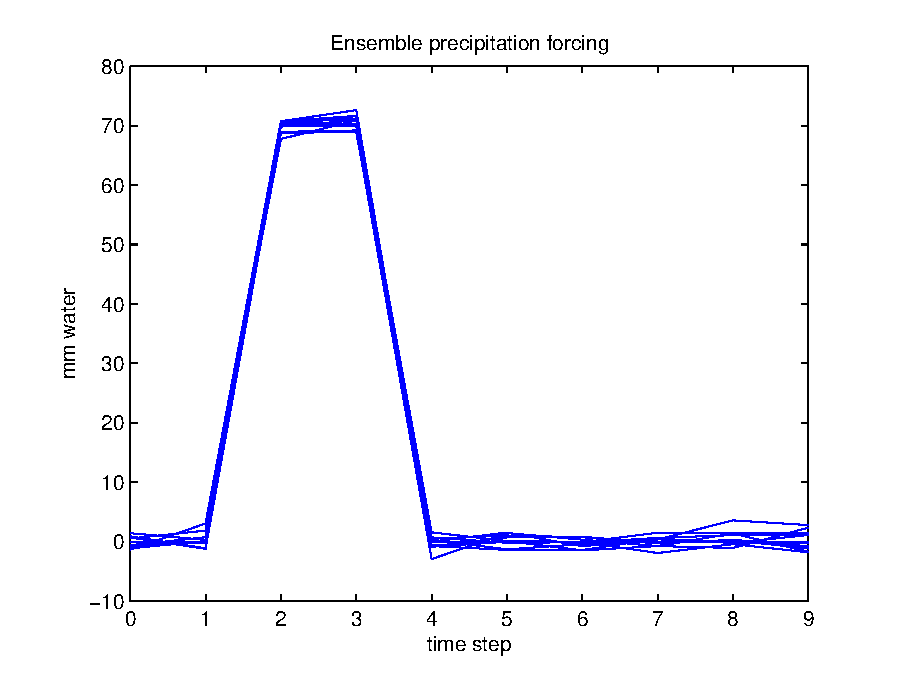
\includegraphics[width=\textwidth]{1b}
      \caption{Nominal precipitation forcing from Problem Set 5.}
      \label{1b}
    \end{figure}
  \item The variance of the error term was chosen to be $\sigma^2_u = 1$. This value implies that approximately 95\% of the forcing are within 2 standard deviations (2mm) of the nominal forcing and, by implication, within that same range of the true value. 
  \item Because it is unlikely that readings from a rain gauge would underestimate the precipitation during a period when the true value is zero, we should question the assumption that the error is unbiased.
    This is especially true of a gauge that can not (or practically does not) indicate negative values. Furthermore, while it is certainly possible to underestimate positive precipitation amounts, this lack of "negative" error should cause us to question the Gaussian assumption as well, even if we postulate a positive bias.
  \item Even if the forcing error may be appropriately considered Gaussian, it relationship with the model is nonlinear and therefore, introduce non-Gaussian error in the model.
\end{itemize}
\subsection{(c)}
\subsection{(a)}
\subsection{(a)}
\subsection{(a)}
\subsection{(a)}
\section{2. Parameter Estimation}
\section{3. Spatially-Homogeneous Force-Restore Model with the EnKF}
\subsection{(a)}
\begin{itemize}
  \item run model
  \item state vector
  \item measurement model
  \item measurement error
  \item mean
  \item covariance 
  \item true precipitation error
\end{itemize}
\subsection{(a)}
\subsection{(a)}
\subsection{(a)}
\section{4. Spatially-Distributed Force-Restore Model with the EnKF}
\subsection{(a)}
\subsection{(a)}
\subsection{(a)}
\subsection{(a)}
\end{document}
